\documentclass{article}
\usepackage{mathtools}
\usepackage{blindtext}
\usepackage{graphicx}
\usepackage{geometry}
\usepackage{ragged2e}
\usepackage[utf8]{inputenc}
\usepackage{xltabular}
\usepackage{booktabs}
\usepackage{titlesec}
\usepackage{hyperref}

\renewcommand{\baselinestretch}{1.3}
\titlespacing\section{0pt}{12pt plus 4pt minus 2pt}{0pt plus 2pt minus 2pt}
\titlespacing\subsection{0pt}{12pt plus 4pt minus 2pt}{0pt plus 2pt minus 2pt}
\titlespacing\subsubsection{0pt}{12pt plus 4pt minus 2pt}{0pt plus 2pt minus 2pt}



\setlength{\parskip}{1em}
\setlength{\parindent}{0pt}
\geometry{
a4paper,
total = {170mm, 257mm},
left = 30mm,
top = 30mm, 
right = 30mm,
bottom = 30mm,
}


\graphicspath{ {images/} }
\title{}
\date{27 de noviembre de 2020}
\begin{document}
\begin{titlepage}
	\centering
	
\includegraphics[width=0.15\textwidth]{uc3m}\par\vspace{1cm}
	{\scshape\LARGE Universidad Carlos III de Madrid \par}
	\vspace{1cm}
	{\scshape\Large Técnicas de Inferencia Estadística II \par}
	\vspace{1.5cm}
	{\huge\bfseries Entrega 1: Análisis Exploratorio de Datos\par}
	\vspace{2cm}
	{\Large\itshape Jorge Salas, Daniel Aramburu y Marc Pastor \par}
	\date{15 de abril de 2020}
	\vfill
	\vfill


% Bottom of the page
	{\large \today\par}
\end{titlepage}

\tableofcontents

\newpage

\section{Introducción}
El objetivo de esta entrega es presentar la base de datos sobre la que trabajaremos durante todo el curso para llevar a cabo contrastes de Hipótesis y practicar la teoría dada en clase. Nuestra objetivo será analizar cómo afecta al precio por noche de los apartamentos de Airbnb de Barcelona las distintas características como: el barrio en el que está situado, el número de habitaciones, la antiguedad del anfitrión, etc.
\section{Dataset}
Hemos obtenido nuestro dataset de \href{http://insideairbnb.com/get-the-data.html}{AirBnb}. Nuestra base de datos está formada por un conjunto de alrededor de 7000 apartamentos de Airbnb de Barcelona con sus respectivas características y variables. Inicialmente partíamos de un conjunto de datos bastante mayor, de alrededor de 21000 filas y 60 variables que tenía el siguiente aspecto:
\vspace{0.45cm}
\begin{figure*}[h]
\hspace*{-0.25cm}
\centering
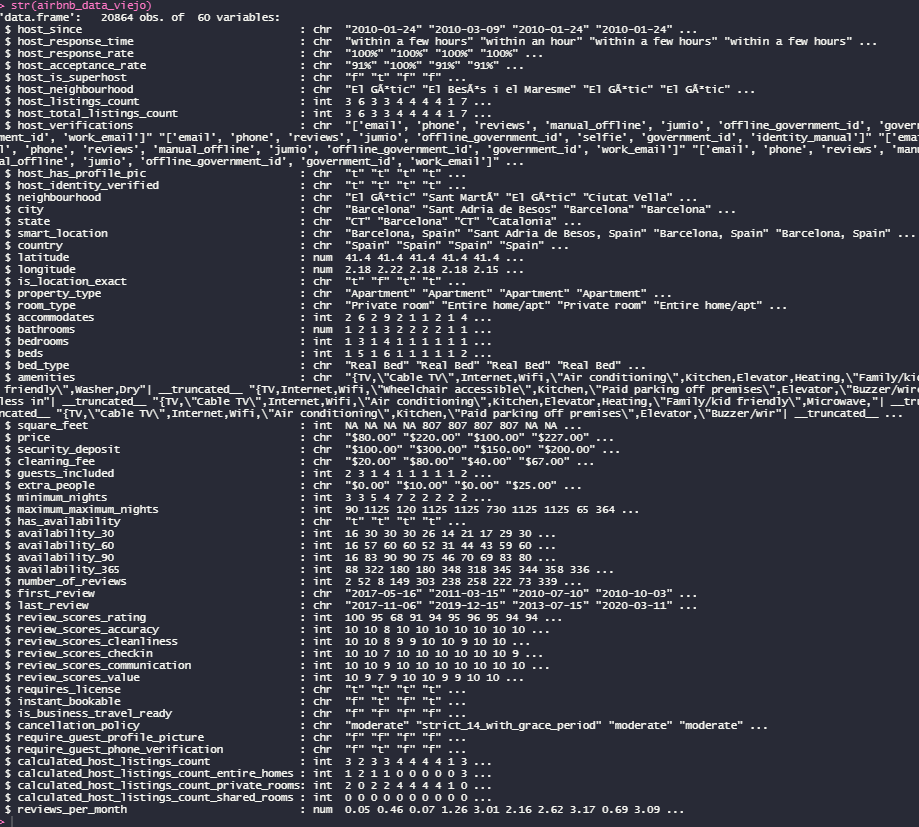
\includegraphics[scale = 0.6]{airbnb_data_viejo}
\end{figure*}

\clearpage
Aplicamos una serie de transformaciones de variables e imputación por mediana (en variables numéricas) y moda (en variables categóricas) para eliminar los NA's el dataset. Finalmente obtenemos el siguiente dataset, ya limpio de NA's.
\vspace{0.45cm}
\begin{figure*}[h]
\hspace*{-0.25cm}
\centering
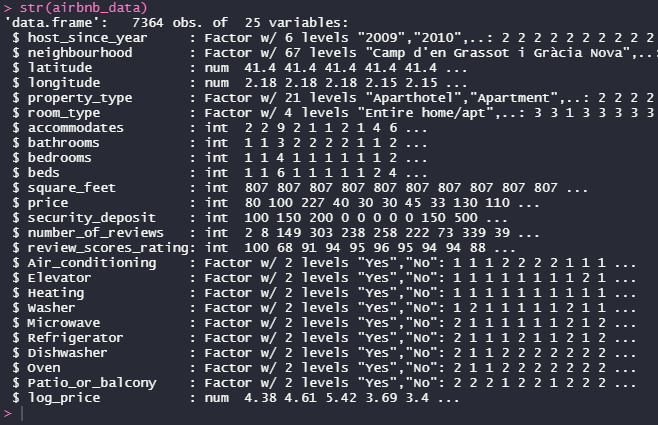
\includegraphics[scale = 0.7]{str_despues}
\end{figure*}

Hemos conseguido eliminar los 61139 NA's que había en los datos:
\vspace{0.45cm}
\begin{figure*}[h]
\hspace*{-0.25cm}
\centering
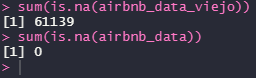
\includegraphics[scale = 0.7]{nas_eliminados}
\end{figure*}

\clearpage
\subsection{Variables}
Nuestro dataset está formado por una muestra 7364 observaciones y 25 variables. Las variables son las siguientes:
\begin{xltabular}{\linewidth}{ l | X | X}
  \caption{Variables de \emph{datos\_airbnb.csv}} 
 \label{table: vardescription}\\
 \hline \hline \hline

\textbf{\normalsize VARIABLE} & \textbf{\normalsize TIPO} & \textbf{\normalsize DESCRIPCIÓN}  \\
 \hline 
\endhead

\textbf{host\_since\_year} & Categórica & Año de registro del anfitrión en Airbnb. \\ \hline 
\textbf{neighbourhood} & Categórica & Barrio en el que se encuentra el apartamento. \\ \hline 
\textbf{latitude} & Numérica & Coordenada de Latitud \\ \hline 
\textbf{longitude} & Numérica & Coordenada de Longitud. \\ \hline 
\textbf{property\_type} & Categórica & Tipo de propiedad.\\ \hline 
\textbf{room\_type} & Categórica & Tipo de habitación. \\ \hline 
\textbf{accommodates} & Numérica & Capacidad de huéspedes. \\ \hline 
\textbf{bathrooms} & Numérica & Número de baños. \\ \hline 
\textbf{bedrooms} & Numérica & Número de dormitorios. \\ \hline 
\textbf{beds} & Numérica & Número de camas. \\ \hline 
\textbf{square\_feet} & Numérica & Superfície del apartamento en $m^{2}$. \\ \hline 
\textbf{price} & Numérica & Precio por noche del apartamento en dólares estadounidenses (\$). \\ \hline 
\textbf{security\_deposit} & Numérica & Fianza en dólares estadounidenses (\$). \\ \hline 
\textbf{number\_of\_reviews} & Numérica & Número de reseñas en Airbnb. \\ \hline 
\textbf{review\_scores\_rating} & Numérica & Puntuación del 1 al 100 en Airbnb. \\ \hline 
\textbf{Air\_Conditioning} & Categórica & Indica si el apartamento dispone de aire acondicionado o no. \\ \hline 
\textbf{Elevator} & Categórica & Indica si el apartamento dispone de ascensor o no. \\ \hline 
\textbf{Heating} & Categórica & Indica si el apartamento dispone de calefacción o no.\\ \hline 
\textbf{Washer} & Categórica &  Indica si el apartamento dispone de lavadora o no. \\ \hline
\textbf{Microwave} & Categórica & Indica si el apartamento dispone de microondas o no. \\ \hline
\textbf{Refrigerator} & Categórica & Indica si el apartamento dispone de nevera o no.  \\ \hline
\textbf{Dishwasher} & Categórica &  Indica si el apartamento dispone de lavavajillas o no. \\ \hline
\textbf{Oven} & Categórica &  Indica si el apartamento dispone de horno o no. \\ \hline
\textbf{Patio\_or\_balcony} & Categórica &  Indica si el apartamento dispone de patio o balcón o no. \\ \hline
\textbf{log\_price} & Numérica &  Logaritmo natural del precio. \\ \hline

\end{xltabular}

\clearpage
\section{Análisis exploratorio de datos}
En este apartado realizamos un análisis exploratorio exhaustivo de las variables, mediante el uso de histogramas, gráficos de barras, tablas y mapas.
\subsection{Variables categóricas}
\subsubsection{\emph{host\_since\_year}}
En este primer gráfico podemos ver en qué año se inscribieron los anfitriones de Airbnb de Barcelona.

\vspace{0.35cm}
\begin{figure*}[h]
\hspace*{-0.15cm}
\centering
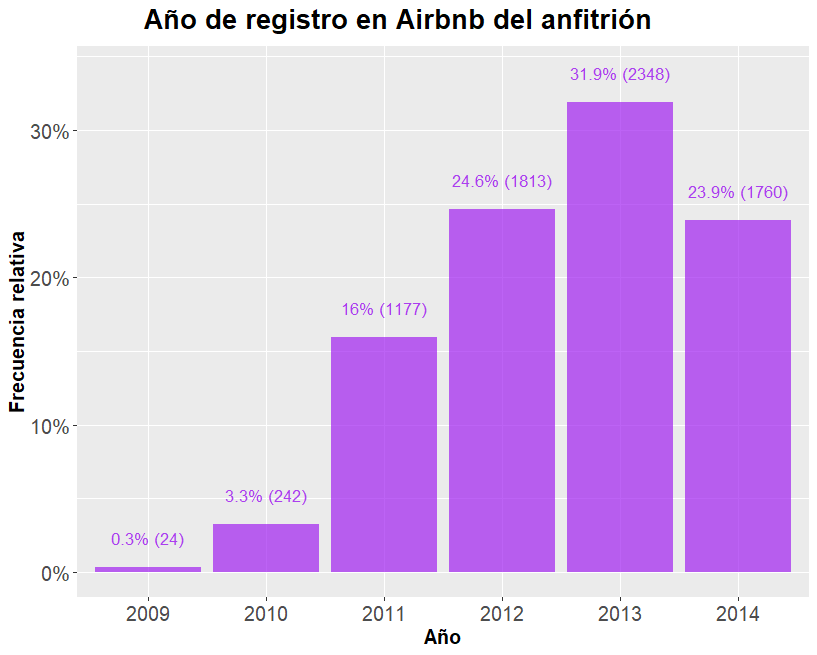
\includegraphics[scale = 0.6]{host_since_year}
\end{figure*}
\vspace{0.35cm}

Como podemos comprobar en el gráfico, los dos primeros años, 2009 y 2010, tuvieron registros mínimos, con tan solo 0.3\% y 3.3\%, principalmente debido a la reciente fundación de Airbnb (2008). A partir del año 2011 se puede apreciar un aumento notable de registros, superando ya el millar y alcanzando máximo en 2013, año en que se registró el 31.9\% de los anfitriones de la muestra. Por el contrario, el último año que fue 2014 redujo sus registros hasta un 23.9\%


\clearpage
\subsubsection{\emph{neighbourhood}}
En este primer \href{https://rpubs.com/marctotti5/754602}{mapa (click para ver la versión interactiva)} podemos observar el número de apartamentos por barrio en la ciudad de Barcelona:

\vspace{0.35cm}
\begin{figure*}[h]
\hspace*{-0.15cm}
\centering
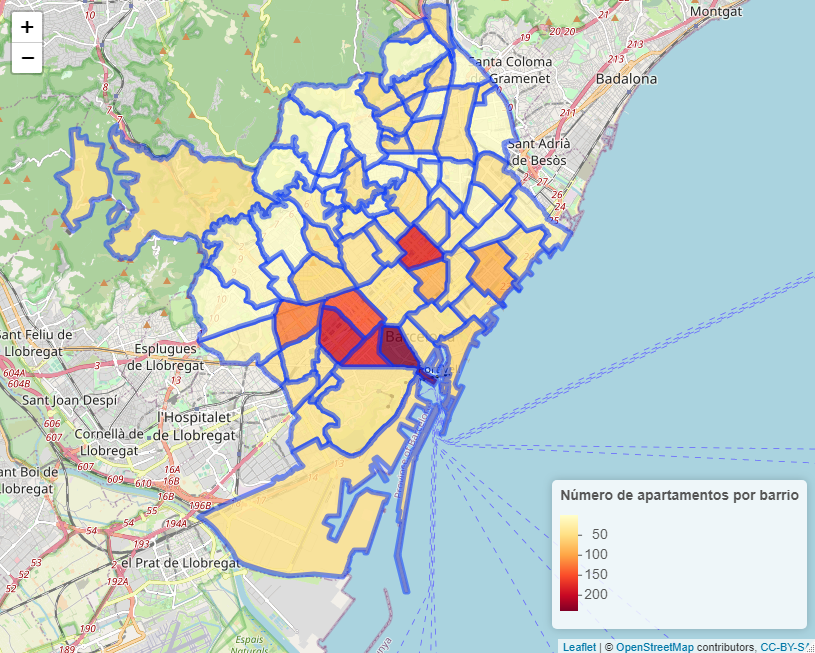
\includegraphics[scale = 0.7]{grafico_3}
\end{figure*}
\vspace{0.35cm}

La zona más concurrida en cuanto a apartamentos se encuentra en el centro de la ciudad, cerca de atracciones turísticas como Plaza Catalunya y Paseo de Gracia, así como en la zona de la Sagrada Família más al norte. El barrio que cuenta con más apartamentos de Airbnb es el Raval, un barrio obrero en las inmediaciones de Plaza Cataluña, conocido por tener una gran comunidad extranjera. 

\clearpage
\subsubsection{\emph{property\_type}}
En este \href{https://rpubs.com/marctotti5/754319}{mapa (click para ver la versión interactiva)} podemos observar los tipos de apartamentos que se ofertan en Airbnb en la ciudad de Barcelona:

\vspace{0.35cm}
\begin{figure*}[h]
\hspace*{-0.15cm}
\centering
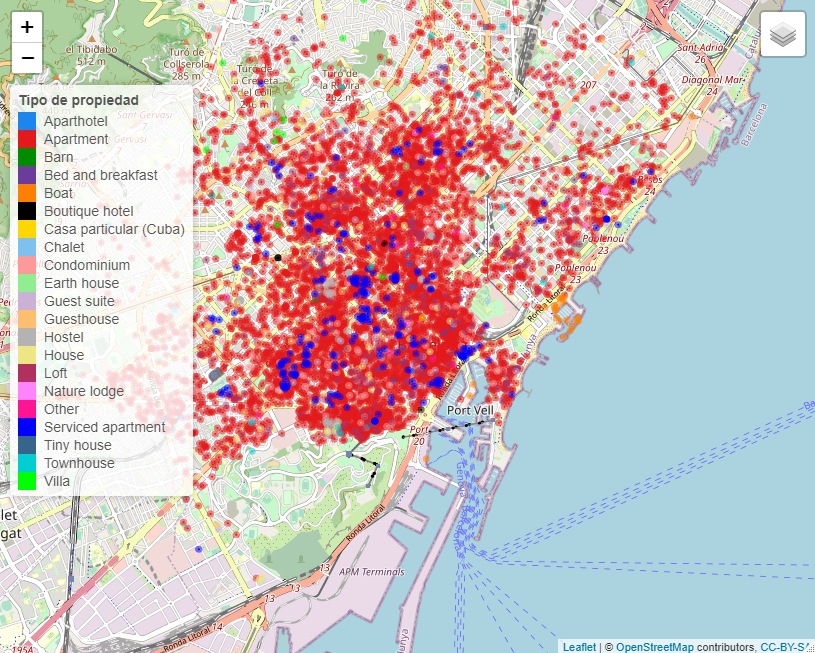
\includegraphics[scale = 0.7]{type_of_property}
\end{figure*}
\vspace{0.35cm}

Se puede ver claramente que la mayoría de ofertas en la web son apartamentos tradicionales (86\%), aunque cabe destacar la presencia de apartamentos con servicios (3.5\%) y también de los lofts. Además es interesante ver que incluso se alquilan barcos enteros así como habitaciones de hotel desde la misma plataforma.

\clearpage
\subsubsection{room\_type}
En este \href{https://rpubs.com/marctotti5/754608}{mapa (click para ver la versión interactiva)} podemos observar los tipos de habitación que se ofrecen en Airbnb en la ciudad de Barcelona:

\vspace{0.35cm}
\begin{figure*}[h]
\hspace*{-0.15cm}
\centering
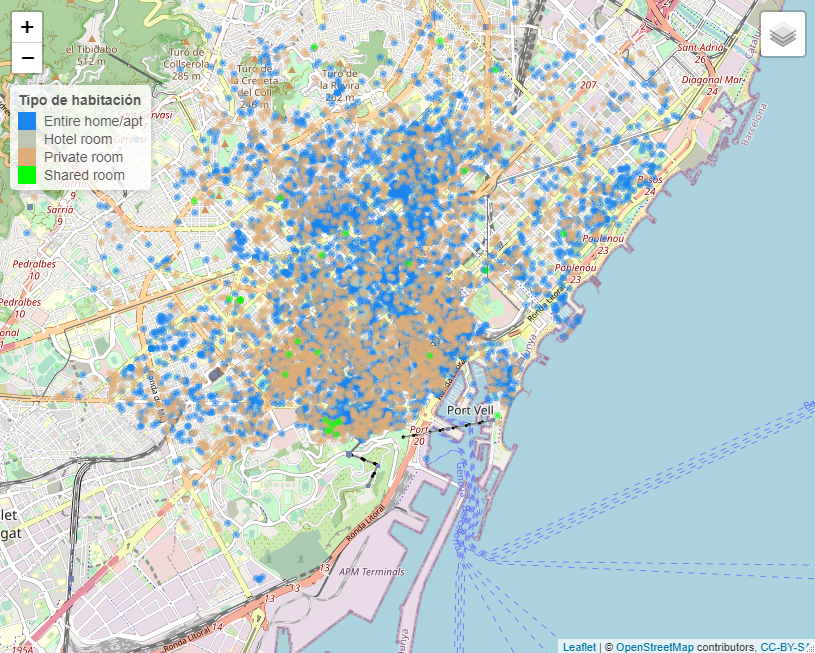
\includegraphics[scale = 0.4]{room_type}
\end{figure*}
\vspace{0.35cm}

Podemos ver como en la zona sur, en barrios cercanos al centro, dominan las habitaciones particulares de alquiler, mientras que en las zonas norte y más alejadas del centro, los apartamentos enteros dominan claramente.

\vspace{0.35cm}
\begin{figure*}[h]
\hspace*{-0.15cm}
\centering
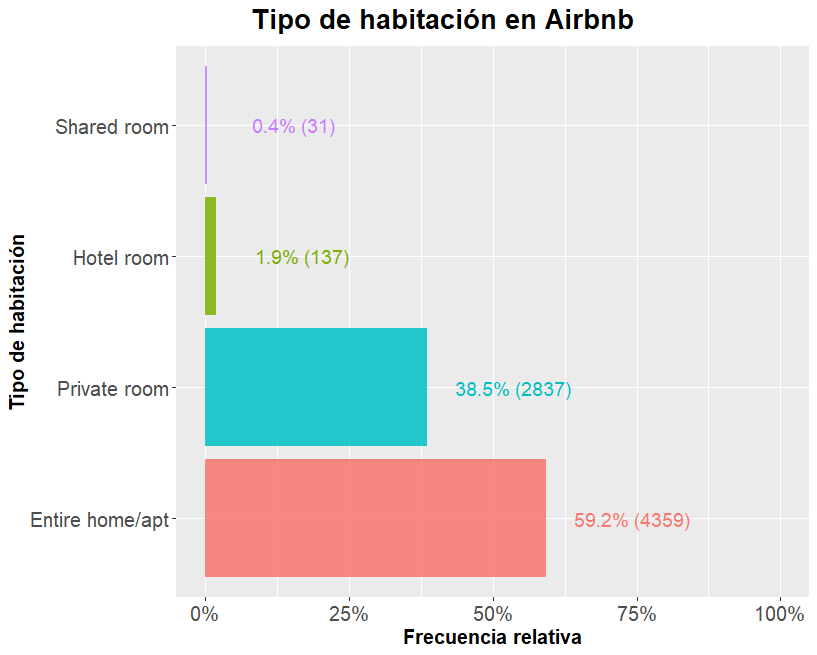
\includegraphics[scale = 0.5]{gráfico_room_type}
\end{figure*}
\vspace{0.15cm}
Además, como podemos ver en el gráfico de barras anterior, la mayoría de anuncios corresponden con apartamentos enteros (59.2\%), aunque las habitaciones privadas tienen mucho peso, principalmente en zonas céntricas, debido probablemente a su menor coste.

\clearpage
\subsubsection{Variables binarias}
A continuación analizamos conjuntamente las variables binarias (\emph{Air\_Conditioning, Elevator, Heating, ...})  ya que solamente toman dos valores: \emph{Yes} o \emph{No}.

\begin{xltabular}{\linewidth}{ l | X | X}
  \caption{Variables binarias} 
 \label{table: vardescription}\\
 \hline \hline \hline

\textbf{\normalsize VARIABLE} & \textbf{\normalsize YES} & \textbf{\normalsize NO}  \\
 \hline 
\endhead

\textbf{Air\_conditioning} & 67.21\% & 32.79\% \\ \hline 
\textbf{Elevator} & 59.13\% & 40.87\% \\ \hline 
\textbf{Heating} & 85.06\% & 14.94\% \\ \hline 
\textbf{Washer} & 84.11\% & 15.89\% \\ \hline 
\textbf{Microwave} & 54.25\% & 45.75\%\\ \hline 
\textbf{Refrigerator} & 59.30\% & 40.70\% \\ \hline 
\textbf{Dishwasher} & 28.06\% & 71.94\% \\ \hline 
\textbf{Oven} & 44.20\% & 55.80\% \\ \hline 
\textbf{Patio\_or\_balcony} & 34.00\% & 66.00\% \\ \hline 
\end{xltabular}

En esta tabla, se puede comprobar cuáles son las características más comunes en los apartamentos de Airbnb. Las más presentes son la calefacción y la lavadora, seguidas por el aire acondicionado. La presencia de ascensor, el microondas y la nevera son aquellos electrodomésticos cuyo porcentaje de presencia  está equilibrada, con alrededor de un 50\%. Por último, las tres variables menos comunes son el horno, el lavavajillas, y el patio o terraza.

\clearpage
\subsection{Variables numéricas}
\subsubsection{\emph{accommodates}}
En este apartado analizamos la capacidad de huéspedes de los apartamentos de Airbnb de Barcelona.

\vspace{0.35cm}
\begin{figure*}[h]
\hspace*{-0.15cm}
\centering
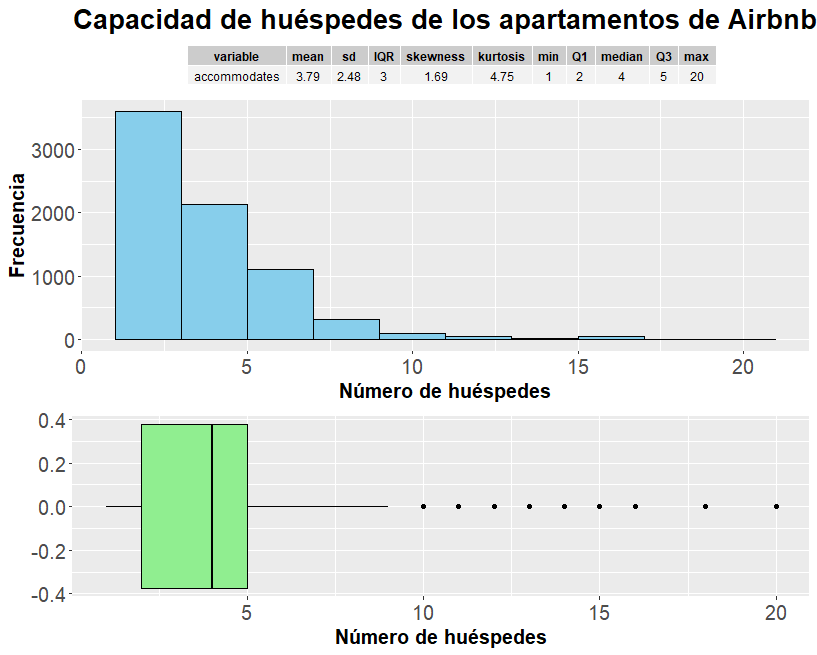
\includegraphics[scale = 0.6]{grafico_accommodates}
\end{figure*}
\vspace{0.15cm}

La media de huéspedes permitidos en los alojamientos es de 3.79, es decir, que está entre 3 y 4 pero hay más alojamientos de 4 huéspedes.
Sd (desviación típica) es 2.48, que se refiere a lo que se suele alejar de la media cualquier dato.
El IQR (Rango Intercuartílico) es de 3, esto quiere decir que la diferencia entre el 25\% y el 75\% de los datos es de 3.
Skewness se refiere al coeficiente de asimetría. Si éste es mayor que 0 significa que la distribución que siguen los datos es asimétrica positiva o a la derecha, más datos mientras más cerca del 0, y viceversa si es menor que 0 , llamándose asimétrica negativa o a la izquierda. Cuando es 0 o muy cercano se puede considerar que es simétrica. En este caso al ser 1.69 significa que los datos son asimétricos positivos.

La curtosis es una medida de forma, es decir, intenta ver a qué se parece la distribución que siguen los datos de la muestra. Si es mayor que 0 se dice que es leptocúrtica (con muchos datos en la media y con las colas, los datos más alejados de la media, con más frecuencia que la distribución normal). En este caso es asimétrica positiva (4.75).
Las que quedan son medidas de dispersión, que son las que dan información acerca de las posiciones relativas de los datos de la muestra. (Q1 y Q3 son las medidas del 25\% y el 75\%, respectivamente, antes explicadas, y la mediana sería Q2, el dato que deja a izquierda y derecha el 50\% de los datos). Para comprobar estos datos véase la tabla situada sobre los gráficos.

\clearpage
\subsection{\emph{bathrooms}}
En este apartado analizamos el número de baños de los apartamentos de Airbnb de Barcelona.

\vspace{0.35cm}
\begin{figure*}[h]
\hspace*{-0.15cm}
\centering
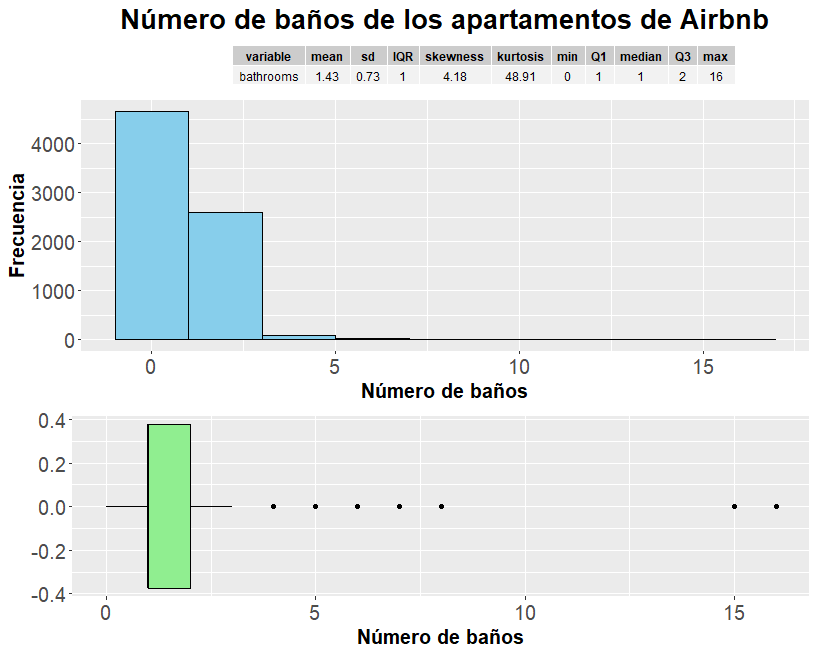
\includegraphics[scale = 0.6]{grafico_bathrooms}
\end{figure*}
\vspace{0.15cm}

La media de baños es de 1.43, es decir, que está entre 1 y 2.
La desviación típica es de 0.79, esto quiere decir que no hay mucha variabilidad en los datos.
El IQR es de 1, lo cual tiene sentido porque suelen haber 1 o 2 baños.
El coeficiente de asimetría es 4.18, así que la distribución es asimétrica positiva.
La curtosis es muy alta así que es muy leptocúrtica (prácticamente todos los datos están en la media).

\clearpage
\subsection{\emph{bedrooms}}
En este apartado analizamos el número de dormitorios de los apartamentos de Airbnb de Barcelona.

\vspace{0.35cm}
\begin{figure*}[h]
\hspace*{-0.15cm}
\centering
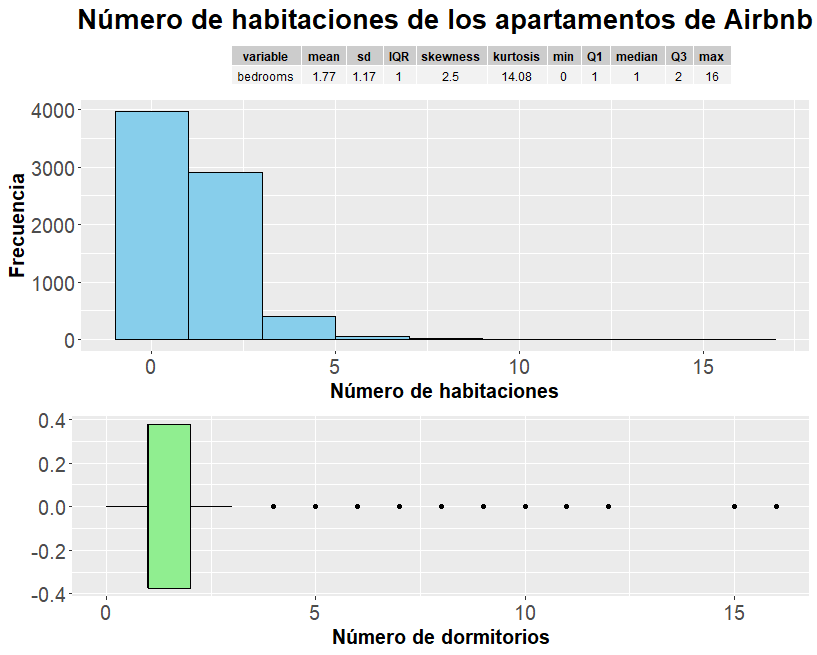
\includegraphics[scale = 0.6]{grafico_bedrooms}
\end{figure*}
\vspace{0.15cm}

La media de dormitorios es de 1.77, es decir, que está entre 1 y 2 pero más cerca de 2.
La desviación típica es de 1.17, por lo que suele haber entre 1 y 3 dormitorios.
El IQR es de 1, ya que Q1 es 1 y Q3 es 2.
El coeficiente de asimetría es 2.5, así que la distribución es asimétrica positiva.
La curtosis es alta, así que la distribución es leptocúrtica (hay muchos datos en la media).

\clearpage
\subsection{\emph{beds}}
En este apartado analizamos el número de camas de los apartamentos de Airbnb de Barcelona.

\vspace{0.35cm}
\begin{figure*}[h]
\hspace*{-0.15cm}
\centering
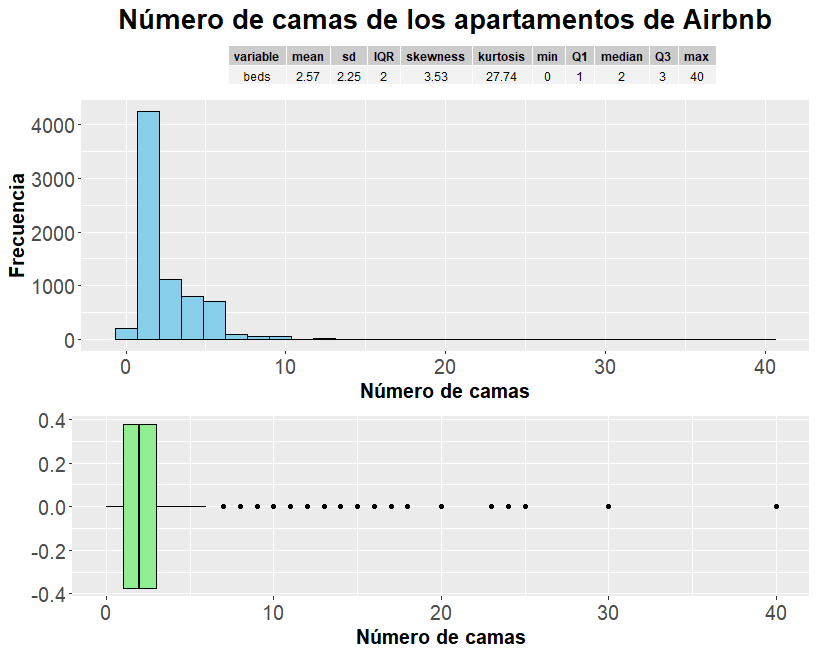
\includegraphics[scale = 0.6]{grafico_beds}
\end{figure*}
\vspace{0.15cm}

La media de camas es de 2.57, es decir, que está entre 2 y 3.
La desviación típica es de 2.25, por lo que suele haber entre 1 y 5 camas.
El IQR es de 2, ya que Q1 es 1 y Q3 es 3.
El coeficiente de asimetría es 3.53, así que la distribución es asimétrica positiva.
La curtosis es alta, así que la distribución es leptocúrtica (hay muchos datos en la media).

\clearpage
\subsection{\emph{square\_feet}}
En este apartado analizamos la superficie en $m^{2}$ de los apartamentos de Airbnb de Barcelona.

\vspace{0.35cm}
\begin{figure*}[h]
\hspace*{-0.15cm}
\centering
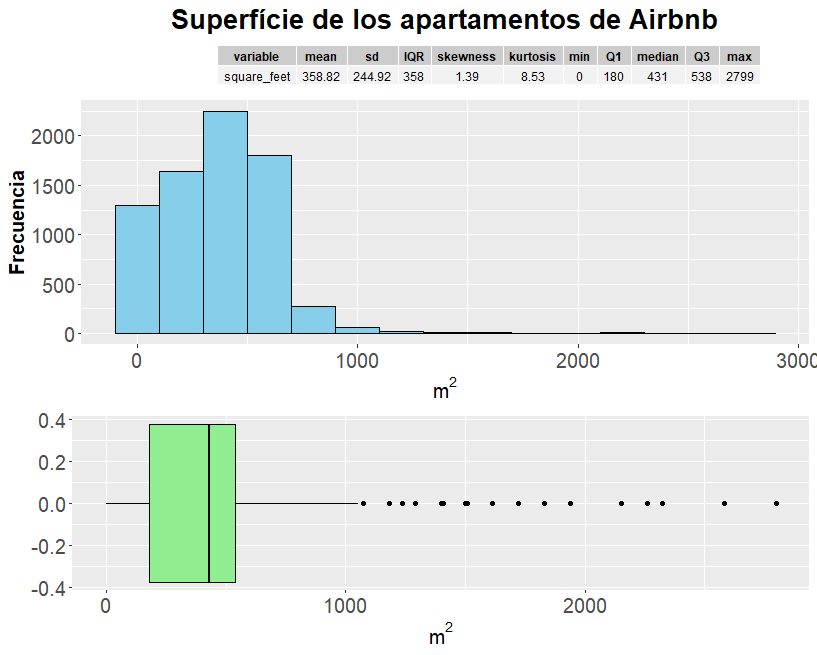
\includegraphics[scale = 0.6]{grafico_square_feet}
\end{figure*}
\vspace{0.15cm}

La media de la superficie de los alojamientos es de 358.82 $m^2$.
La desviación típica es de 244.92 $m^2$, por lo que hay mucha dispersión en los datos.
El IQR es de 358, ya que Q1 es 180 y Q3 es 538, lo que nos da una idea más visual de la dispersión de los datos, ya que entre el primer 25\% de los datos y el 75\% de los datos, hay una diferencia de 358 $m^2$, lo cuál indica que hay pisos de superfícies muy dispares en la ciudad condal.
El coeficiente de asimetría es 1.39, así que la distribución es asimétrica positiva.
La curtosis es alta, así que la distribución es leptocúrtica (hay muchos datos en la media).
El 0 del mínimo es consecuencia de datos atípicos, ya que no tiene sentido.

\clearpage
\subsection{\emph{security\_deposit}}
En este apartado analizamos la fianza en dólares estadounidenses (\$) de los apartamentos de Airbnb de Barcelona. La fianza es un importe que el huésped debe ingresar al arrendador como garantía del buen uso de las instalaciones. En caso de que el inquilino ocasionara algún desperdicio en el apartamento, el anfitrión podría quedarse con dicho importe a modo de indemnización. 

\vspace{0.35cm}
\begin{figure*}[h]
\hspace*{-0.15cm}
\centering
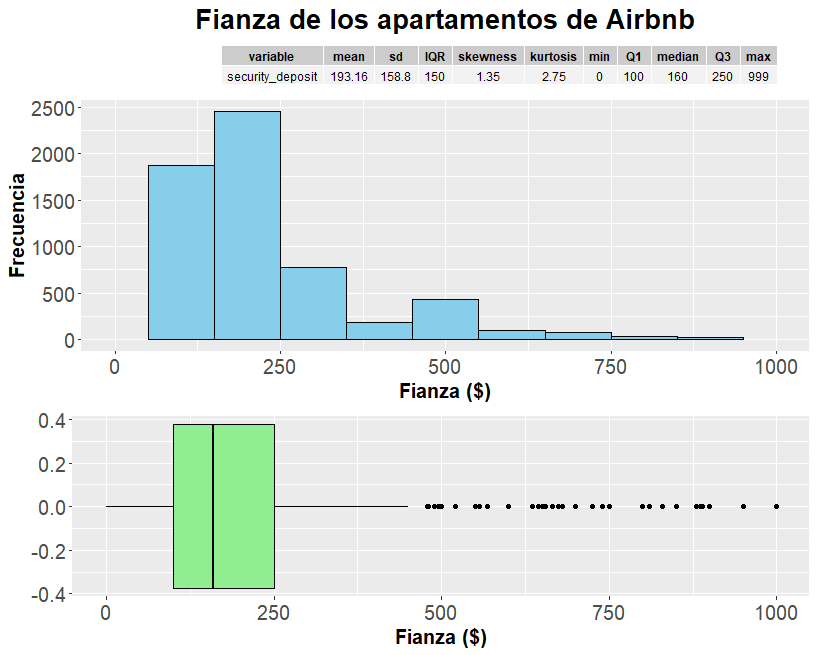
\includegraphics[scale = 0.6]{grafico_security_deposit}
\end{figure*}
\vspace{0.15cm}

La media de las fianzas es de 193.16\$.
La desviación típica es de 158.8\$, lo que indica mucha dispersión.
El IQR es de 150\$, ya que Q1 es 100 y Q3 es 250, lo que también indica bastante variabilidad en los datos.
El coeficiente de asimetría es 1.35, así que la distribución es asimétrica positiva.
La curtosis es alta, así que la distribución es leptocúrtica (hay muchos datos alrededor de la media), es decir la distribución sería más apuntada y con colas más pesadas que la normal.

\clearpage
\subsection{\emph{number\_of\_reviews}}
En este apartado analizamos el número de reseñas online de los apartamentos de Airbnb de Barcelona. 

\vspace{0.35cm}
\begin{figure*}[h]
\hspace*{-0.15cm}
\centering
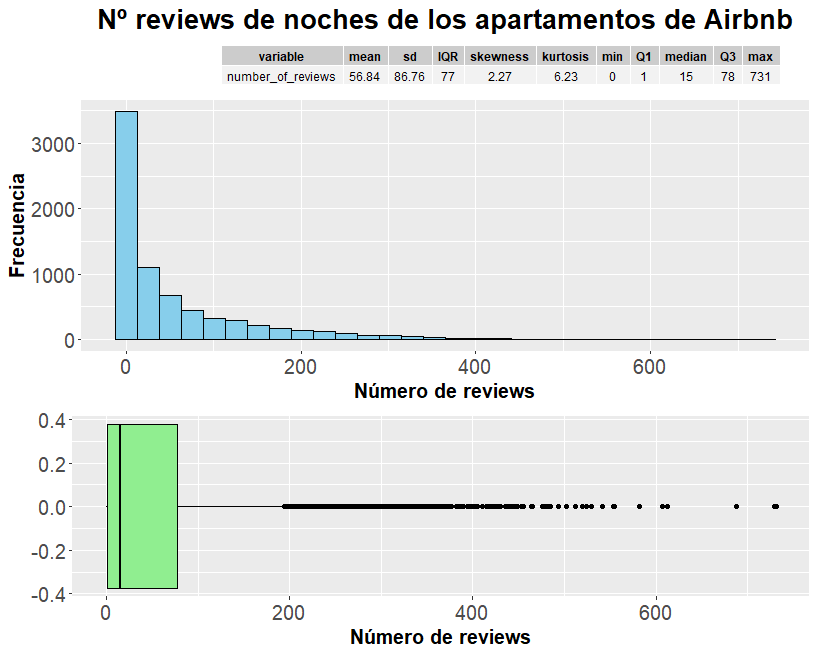
\includegraphics[scale = 0.6]{grafico_number_of_reviews}
\end{figure*}
\vspace{0.15cm}

La media de reviews es de 56.84, es decir, que está entre 56 y 57, pero más cerca de 57.
La desviación típica es de 86.76, es decir, que los datos están muy dispersos.
El IQR es de 77, ya que Q1 es 1 y Q3 es 78, lo que corrobora que la dispersión de los datos.
El coeficiente de asimetría es 2.27, así que la distribución es asimétrica positiva, como se puede ver claramente en el histograma.
La curtosis es positiva, así que la distribución es leptocúrtica (hay más datos en la media que en el resto de la distribución)

\clearpage
\subsection{\emph{review\_scores\_rating}}
En este apartado analizamos la puntuación (del 1 al 100) de los apartamentos de Airbnb de Barcelona. 

\vspace{0.35cm}
\begin{figure*}[h]
\hspace*{-0.15cm}
\centering
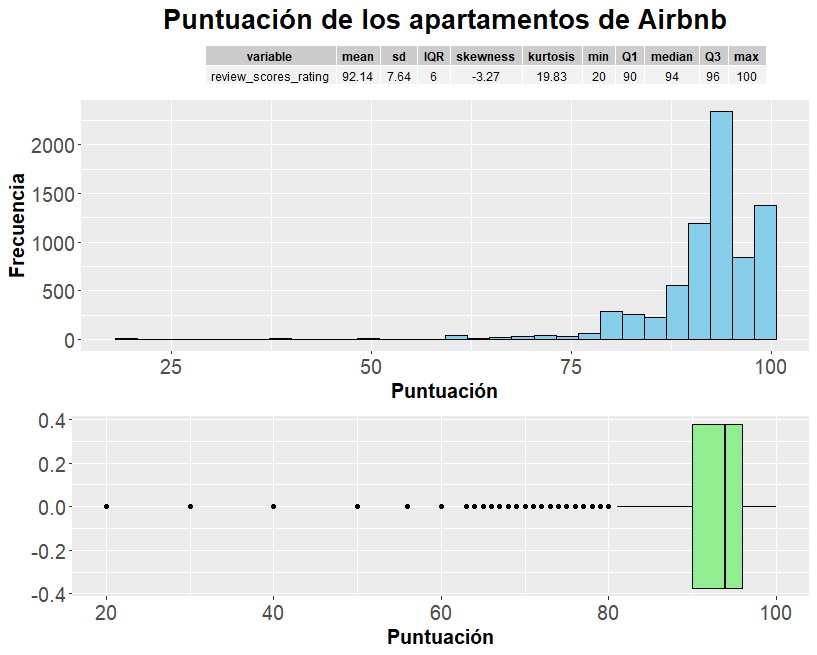
\includegraphics[scale = 0.6]{grafico_scores_rating}
\end{figure*}
\vspace{0.15cm}

La media de la puntuación de los usuarios es de 92.14.
La desviación típica es de 7.64, aunque es un número relativamente alto, es pequeño comparado con el tamaño de los demás así que la dispersión es pequeña.  
El IQR es de 6, ya que Q1 es 90 y Q3 es 96, lo que también indica poca dispersión, demostrando también la poca dispersión.
El coeficiente de asimetría es -3.27, así que la distribución es asimétrica negativa.
La curtosis es bastante alta, así que la distribución es leptocúrtica (hay muchos datos en la media).
Es decir que en general las puntuaciones son muy altas, así que podría ser que los apartamentos realmente fueran muy buenos, o bien que los clientes no son muy críticos y puntúan alto siempre.

\clearpage
\subsection{\emph{price}}
En este apartado analizamos el precio por noche en dólares estadounidenses (\$) de los apartamentos de Airbnb de Barcelona. Esta variable va a ser el \textbf{principal objeto de nuestra investigación} y por ello le prestamos especial atención. 

\vspace{0.35cm}
\begin{figure*}[h]
\hspace*{-0.15cm}
\centering
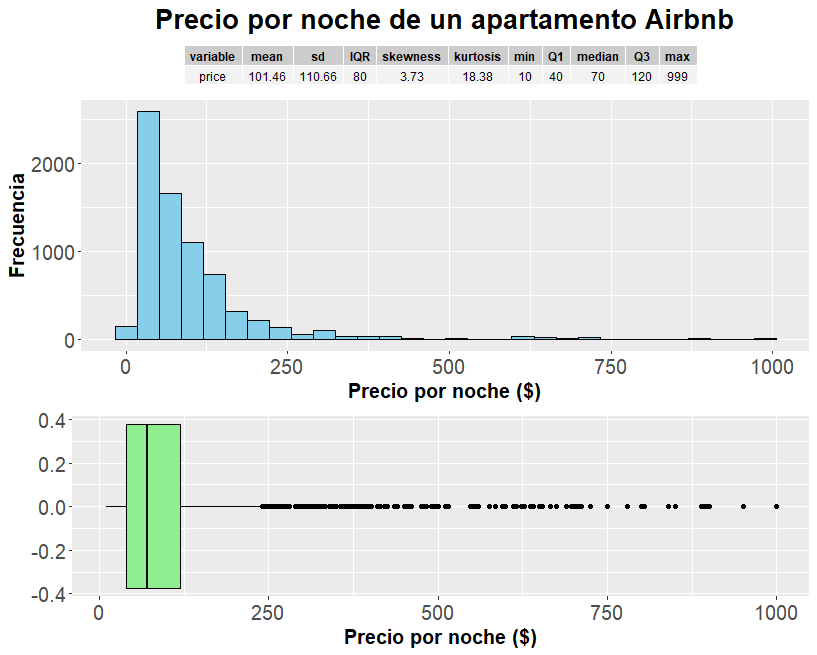
\includegraphics[scale = 0.6]{grafico_precio}
\end{figure*}
\vspace{0.15cm}

La media del precio por noche es de 101.45\$.
La desviación típica es de 110.66\$, lo que indica mucha dispersión en los datos.
El IQR es de 80, ya que Q1 es 40 y Q3 es 120, lo que también indica bastante dispersión entre los pisos más baratos y caros. Es decir entre el 25\% de pisos más baratos y el 75\% hay una diferencia de 80\$.
El coeficiente de asimetría es 3.73, por lo que se podría decir que la distribución es asimétrica positiva, y por ende no tiene un aspecto muy gaussiano (no parece que siga una distribución normal), lo cuál podría suponer un problema al violar los supuestos necesarios para realizar muchos contrastes de hipótesis. 
La curtosis es 18.38, es decir, la distribución no tiene nada que ver con una normal, ya que es mucho más apuntada y con colas más pesadas. A priori podríamos pensar en que los datos podrían seguir una distribución log-normal, o una gamma. 

\clearpage
Debido a que estamos interesados la normalidad de los datos, llevamos a cabo una transformación logarítmica de la variable \emph{price}, obteniendo así una variable llamada \emph{log\_price}. A continuación la analizamos:

\vspace{0.35cm}
\begin{figure*}[h]
\hspace*{-0.15cm}
\centering
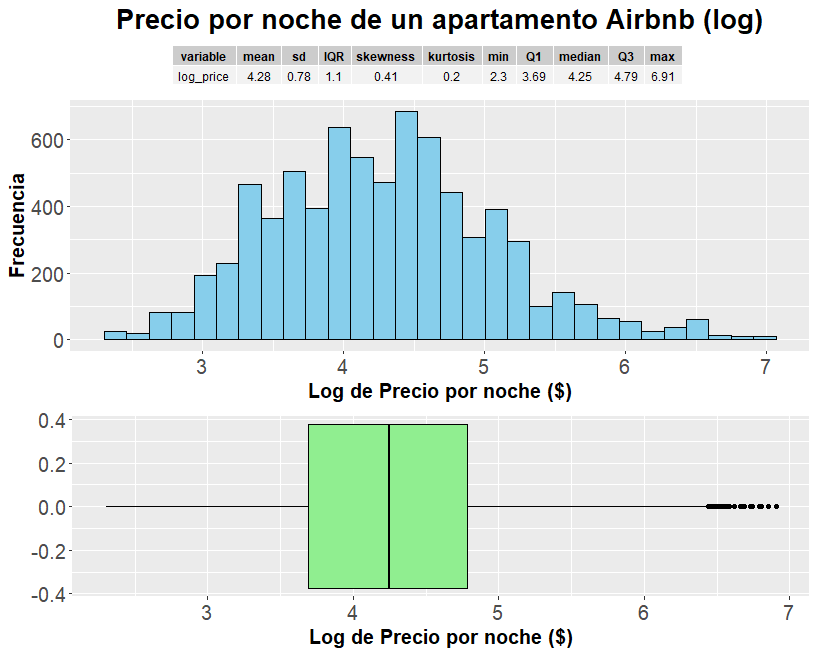
\includegraphics[scale = 0.6]{grafico_precio_log}
\end{figure*}
\vspace{0.15cm}

Estos datos nos permiten ver claramente que el logaritmo del precio tendría mucha menos variabilidad, y estaría mucho más cerca de seguir una distribución normal. Los coeficientes de asimetría y kurtosis indican que la distribución es prácticamente simétrica y muy parecida a una normal. Es por ello que nos planteamos usar esta variable para realizar los contrastes de hipótesis relativos al precio.

\clearpage
A continuación analizamos la relación del precio con el resto de variables cualitativas y numéricas:
\subsubsection{\emph{price} y \emph{host\_since\_year}}

En este gráfico podemos observar el precio por noche según la antigüedad del anfitrión de la ciudad:

\vspace{0.35cm}
\begin{figure*}[h]
\hspace*{-0.15cm}
\centering
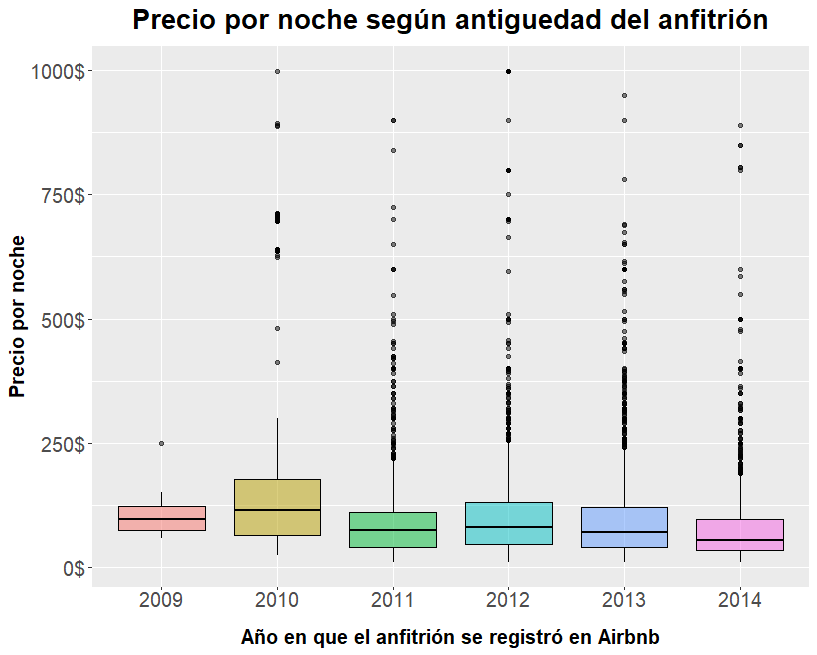
\includegraphics[scale = 0.6]{boxplot_precio_antiguedad}
\end{figure*}
\vspace{0.15cm}

Este gráfico muestra como los anfitriones de 2010 tienen el mayor precio promedio por noche, aunque la diferencia podría ser no significativa estadísticamente. Cabe destacar que en todos los años hay gran cantidad de datos atípicos y que habría que contrastar si las diferencias de precio son significativas o no.

\clearpage
\subsubsection{\emph{price} y \emph{neighbourhood}}

En este \href{https://rpubs.com/marctotti5/754320}{gráfico (click para ver la versión interactiva)} podemos observar el precio medio por barrio de la ciudad:
\vspace{0.35cm}
\begin{figure*}[h]
\hspace*{-0.15cm}
\centering
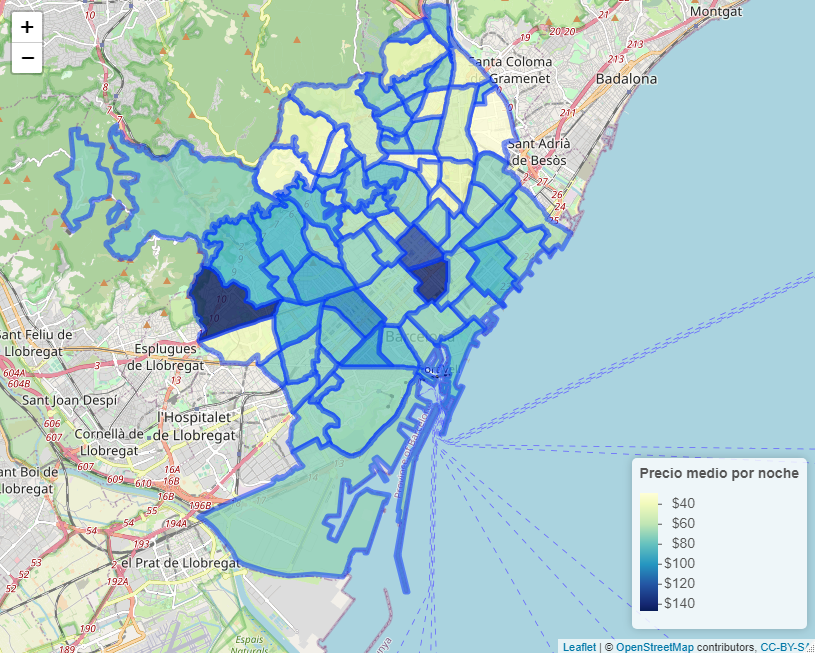
\includegraphics[scale = 0.6]{price_per_neighbourhood}
\end{figure*}
\vspace{0.15cm}

Podemos ver que las zonas más cotizadas estarían en la zona alta de Barcelona (Pedralbes y Sant Gervasi), tradicionalmente barrios en los que vive la gente con mayor poder adquisitivo de la ciudad, con un precio medio por noche de 143\$. Si recordamos del mapa de apartamentos por barrio éste no destacaba por disponer de una gran oferta, ya que la mayoría se encontraban en zonas céntricas como \emph{el Raval} y la Sagrada Familia. Por otro lado, cabe destacar la zona del Fort Pienc, cerca del distrito financiero de la ciudad que sería la segunda más cara, con un precio medio de 143\$ por noche. Finalmente, las zonas periféricas y tradicionalmente más conflictivas forman una alternativa más económica, con precios que van entre 25 y 40\$ por noche de media.

\clearpage
\subsubsection{\emph{price} y \emph{property\_type}}

En este gráfico podemos observar el precio medio por noche de Airbnb en función del tipo de propiedad:

\vspace{0.35cm}
\begin{figure*}[h]
\hspace*{-0.15cm}
\centering
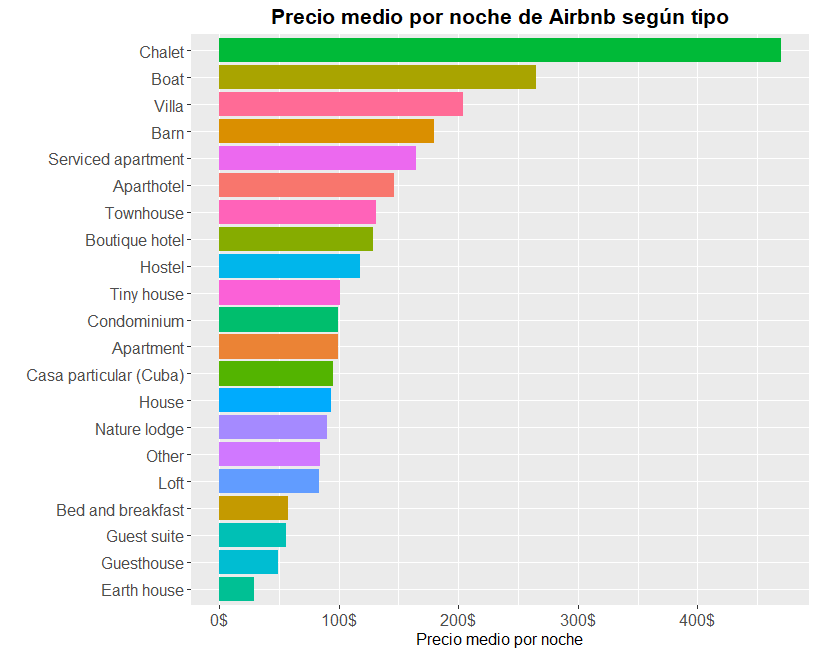
\includegraphics[scale = 0.6]{precio_tipo_propiedad}
\end{figure*}
\vspace{0.15cm}

En este caso podemos ver que existen claras diferencias en el precio promedio por noche en función del tipo de propiedad. Las propiedades más caras de alquilar serían los chalets (posiblemente debido a su mayor superficie, capacidad de huéspedes y ubicación), los barcos y las villas. Los apartamentos tradicionales tendrían un precio promedio más accesible para la mayor parte de la población, de alrededor de 100\$ por noche, lo cuál explicaría su clamoroso éxito. Sería interesante contrastar el precio promedio mediante un análisis de la varianza para observar si estas diferencias son significativas. 

\clearpage
\subsubsection{\emph{price} y \emph{room\_type}}

En este gráfico podemos observar el precio medio por noche de Airbnb en función del tipo de habitación:

\vspace{0.35cm}
\begin{figure*}[h]
\hspace*{-0.15cm}
\centering
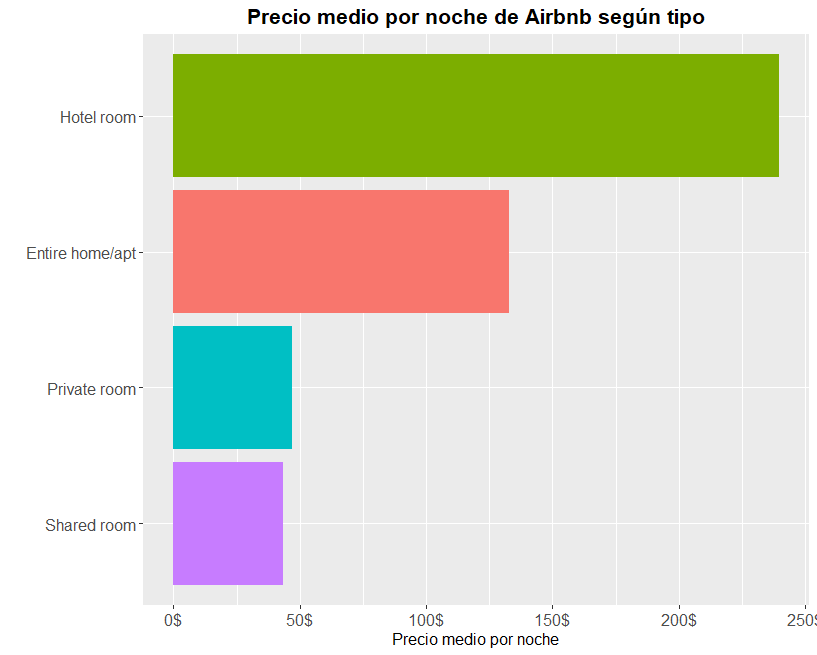
\includegraphics[scale = 0.6]{price_room_type}
\end{figure*}
\vspace{0.15cm}

En este caso podemos ver que existen claras diferencias en el precio promedio por noche en función del tipo de habitación. Las habitaciones de hotel serían las más caras por noche, prácticamente costarían en promedio el doble que dormir en un apartamento entero. Finalmente las alternativas más baratas serían las habitaciones individuales y compartidas, con precios medios de alrededor de 50\$. Sería interesante contrastar estas hipótesis mediante análisis de la varianza y Tukey. 

\clearpage
\subsubsection{\emph{price} y \emph{Air\_Conditioning}}

En este gráfico podemos observar el precio por noche de Airbnb en función de si el apartamento en cuestión dispone de aire acondicionado o no:

\vspace{0.35cm}
\begin{figure*}[h]
\hspace*{-0.15cm}
\centering
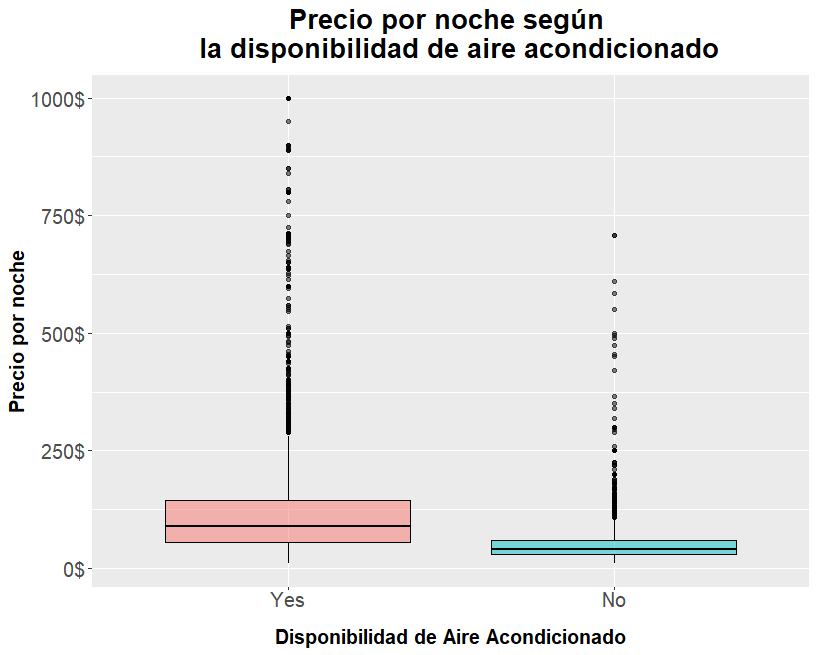
\includegraphics[scale = 0.6]{boxplot_precio_air_conditioning}
\end{figure*}
\vspace{0.15cm}

En este gráfico podemos ver que parece que el precio del alojamiento sube si tiene aire acondicionado, tanto en los que están en un intervalo razonable (la parte coloreada), como los que se alejan de los precios estándar. Habría que contrastar esto rigurosamente.

\clearpage
\subsubsection{\emph{price} y \emph{Elevator}}

En este gráfico podemos observar el precio por noche de Airbnb en función de si el apartamento en cuestión dispone de ascensor o no:

\vspace{0.35cm}
\begin{figure*}[h]
\hspace*{-0.15cm}
\centering
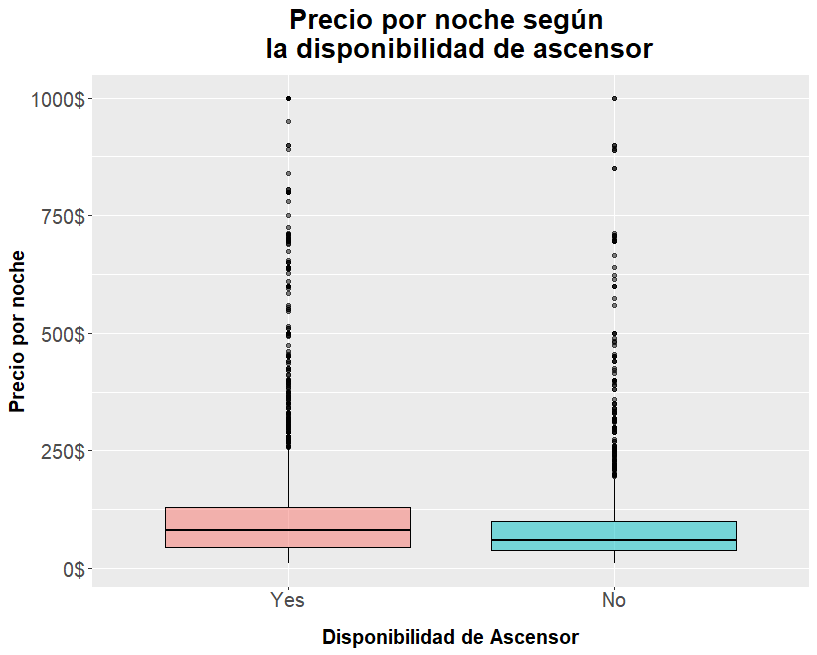
\includegraphics[scale = 0.6]{boxplot_precio_Elevator}
\end{figure*}
\vspace{0.15cm}

En este gráfico podemos ver que parece que el precio del alojamiento sube ligeramente si tiene ascensor, tanto en los que están en un intervalo razonable (la parte coloreada), como los que se alejan de los precios estándar. Habría que contrastar esto rigurosamente, porque probablemente la diferencia no sea significativa estadísticamente.

\clearpage
\subsubsection{\emph{price} y \emph{Heating}}

En este gráfico podemos observar el precio por noche de Airbnb en función de si el apartamento en cuestión dispone de calefacción o no:

\vspace{0.35cm}
\begin{figure*}[h]
\hspace*{-0.15cm}
\centering
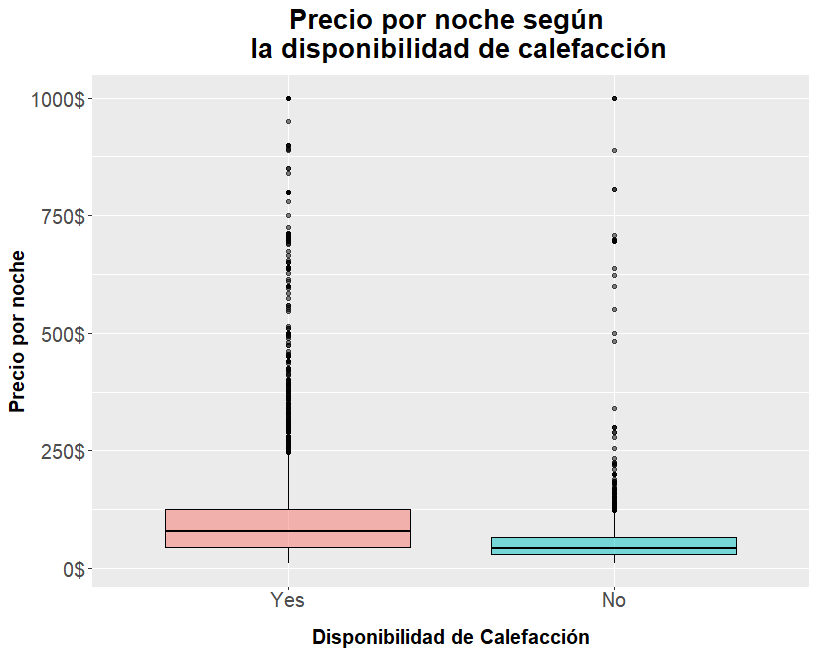
\includegraphics[scale = 0.6]{boxplot_precio_Heating}
\end{figure*}
\vspace{0.15cm}

En este gráfico podemos ver que parece que el precio del alojamiento sube ligeramente si tiene calefacción. Habría que contrastar esto rigurosamente, porque probablemente la diferencia no sea significativa estadísticamente.

\clearpage
\subsubsection{\emph{price} y \emph{Washer}}

En este gráfico podemos observar el precio por noche de Airbnb en función de si el apartamento en cuestión dispone de lavadora o no:

\vspace{0.35cm}
\begin{figure*}[h]
\hspace*{-0.15cm}
\centering
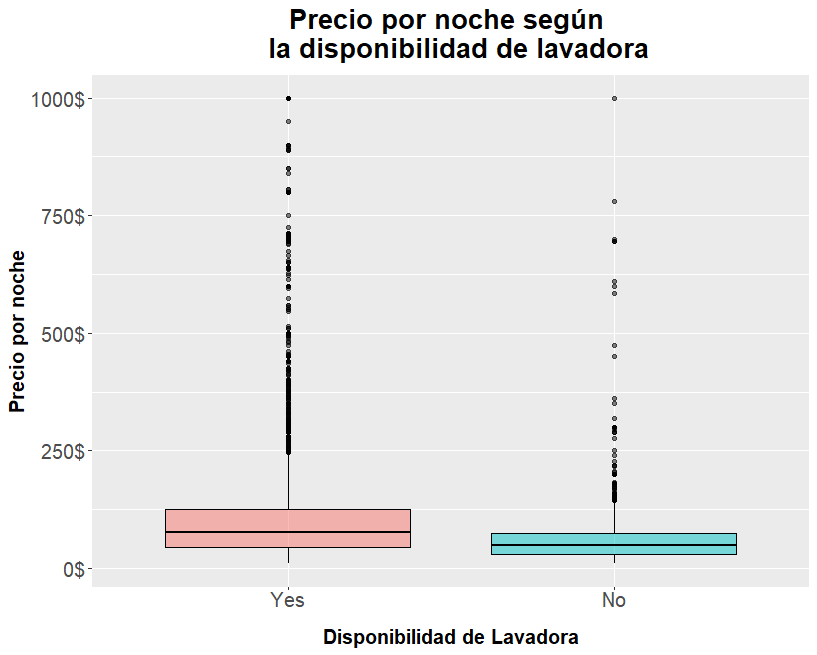
\includegraphics[scale = 0.6]{boxplot_precio_Washer}
\end{figure*}
\vspace{0.15cm}

En este gráfico podemos ver que parece que el precio del alojamiento sube ligeramente si tiene lavadora. Habría que contrastar esto rigurosamente, porque probablemente la diferencia no sea significativa estadísticamente.

\clearpage
\subsubsection{\emph{price} y \emph{Microwave}}

En este gráfico podemos observar el precio por noche de Airbnb en función de si el apartamento en cuestión dispone de microondas o no:

\vspace{0.35cm}
\begin{figure*}[h]
\hspace*{-0.15cm}
\centering
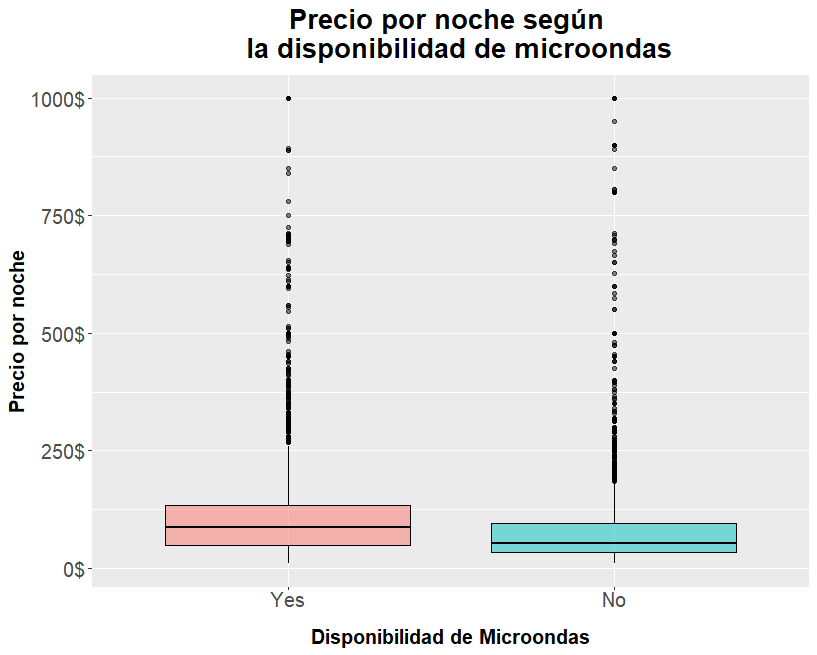
\includegraphics[scale = 0.6]{boxpot_precio_Microwave}
\end{figure*}
\vspace{0.15cm}

En este gráfico podemos ver que parece que el precio del alojamiento sube ligeramente si tiene microondas. Habría que contrastar esto rigurosamente, porque probablemente la diferencia no sea significativa estadísticamente.

\clearpage
\subsubsection{\emph{price} y \emph{Refrigerator}}

En este gráfico podemos observar el precio por noche de Airbnb en función de si el apartamento en cuestión dispone de nevera o no:

\vspace{0.35cm}
\begin{figure*}[h]
\hspace*{-0.15cm}
\centering
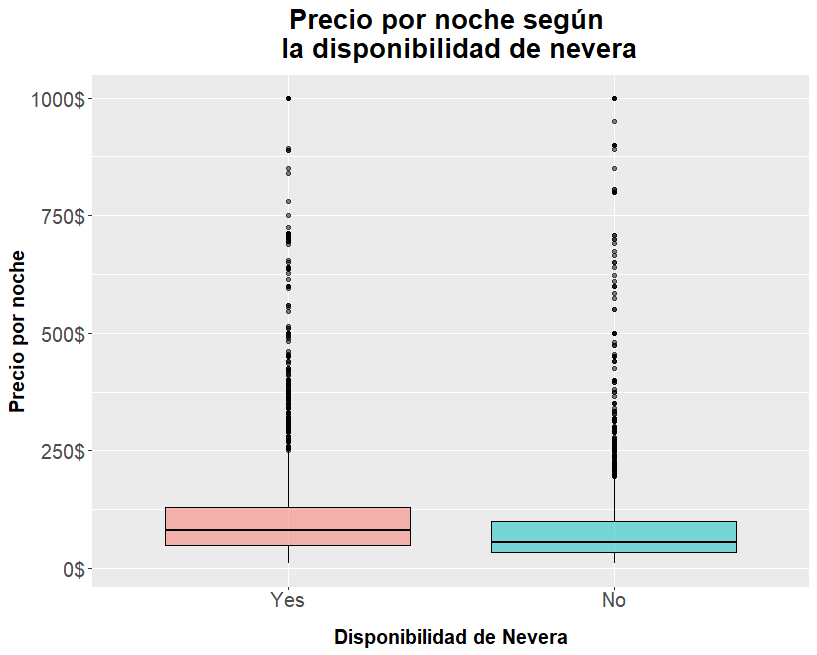
\includegraphics[scale = 0.6]{boxplot_precio_Refrigerator}
\end{figure*}
\vspace{0.15cm}

En este gráfico podemos ver que parece que el precio del alojamiento sube ligeramente si tiene nevera. Habría que contrastar esto rigurosamente, porque probablemente la diferencia no sea significativa estadísticamente.

\clearpage
\subsubsection{\emph{price} y \emph{Dishwasher}}

En este gráfico podemos observar el precio por noche de Airbnb en función de si el apartamento en cuestión dispone de lavavajillas o no:

\vspace{0.35cm}
\begin{figure*}[h]
\hspace*{-0.15cm}
\centering
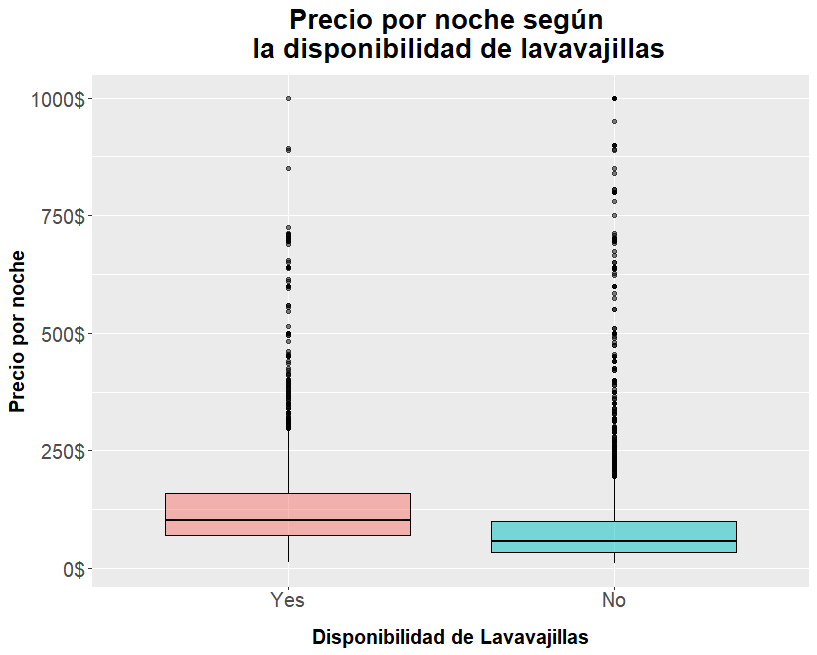
\includegraphics[scale = 0.6]{boxplot_precio_Dishwasher}
\end{figure*}
\vspace{0.15cm}

En este gráfico podemos ver que parece que el precio del alojamiento sube ligeramente si tiene lavavajillas. Habría que contrastar esto rigurosamente, porque probablemente la diferencia no sea significativa estadísticamente.

\clearpage
\subsubsection{\emph{price} y \emph{Oven}}

En este gráfico podemos observar el precio por noche de Airbnb en función de si el apartamento en cuestión dispone de horno o no:

\vspace{0.35cm}
\begin{figure*}[h]
\hspace*{-0.15cm}
\centering
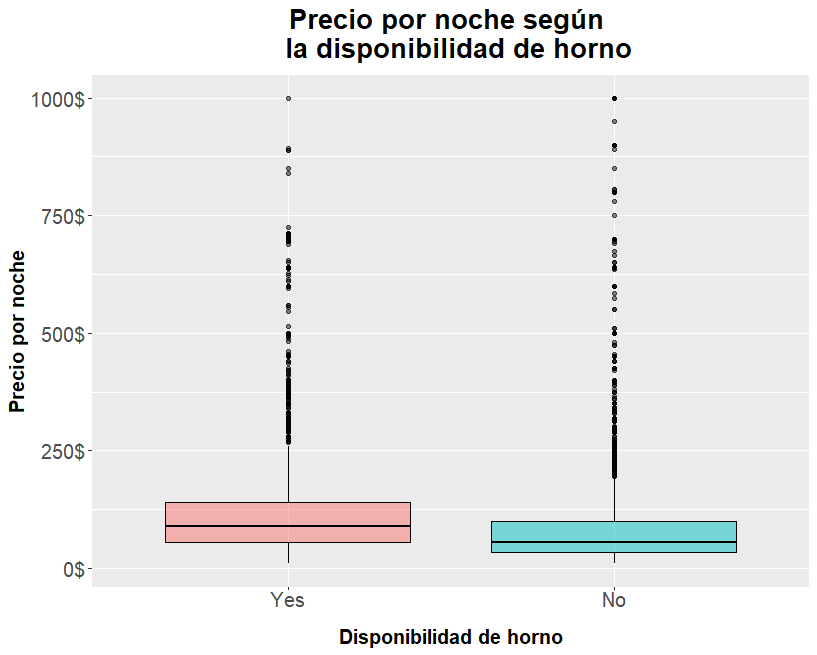
\includegraphics[scale = 0.6]{boxplot_precio_Oven}
\end{figure*}
\vspace{0.15cm}

En este gráfico podemos ver que parece que el precio del alojamiento sube ligeramente si tiene horno. Habría que contrastar esto rigurosamente, porque probablemente la diferencia no sea significativa estadísticamente.

\clearpage
\subsubsection{\emph{price} y \emph{Patio\_or\_balcony}}

En este gráfico podemos observar el precio por noche de Airbnb en función de si el apartamento en cuestión dispone de patio o balcón o no:

\vspace{0.35cm}
\begin{figure*}[h]
\hspace*{-0.15cm}
\centering
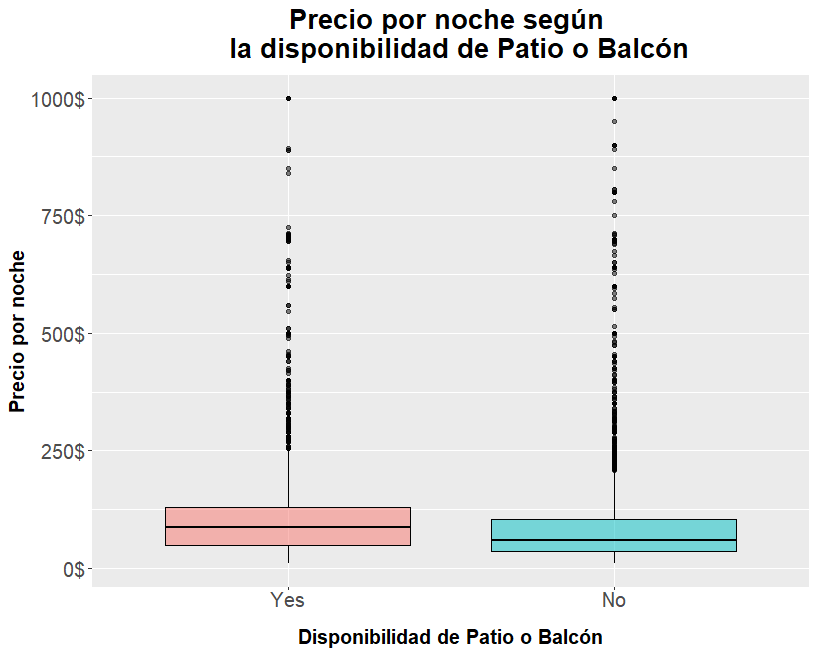
\includegraphics[scale = 0.6]{boxplot_precio_Patio_or_balcony}
\end{figure*}
\vspace{0.15cm}

En este gráfico podemos ver que parece que el precio del alojamiento sube ligeramente si tiene patio o balcón. Habría que contrastar esto rigurosamente, porque probablemente la diferencia no sea significativa estadísticamente.

\clearpage
\subsubsection{Relación del precio con las demás variables numéricas}

En este gráfico podemos observar los coeficientes de correlaciones de Pearson del precio con las demás variables numéricas:

\vspace{0.35cm}
\begin{figure*}[h]
\hspace*{-0.15cm}
\centering
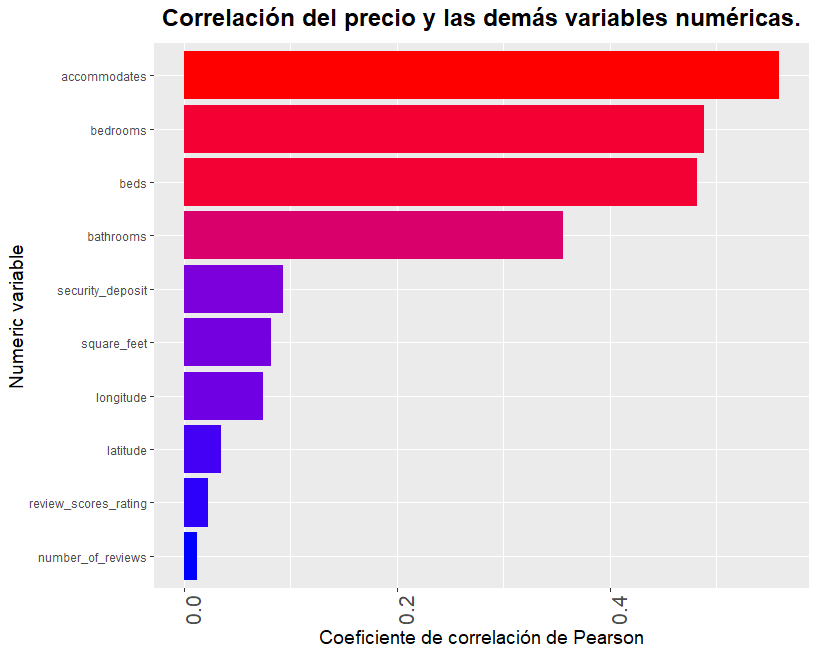
\includegraphics[scale = 0.6]{grafico_correlaciones_pearson}
\end{figure*}
\vspace{0.15cm}

La variable que más influiría en el precio sería la capacidad de huéspedes, con una correlación de 0.55, seguida del número de dormitorios y de camas. Por otro lado cabe destacar que el precio parece no mantener relación con el número de reviews o la puntuación del apartamento en cuestión, y relativamente poca correlación con la superfície del sitio.


\clearpage
\section{Bibliografía}
1. \emph{Datos de Airbnb Barcelona} Datos recuperados de http://insideairbnb.com/get-the-data.html














































\end{document}
